\subsection{Analyse Otto}
Mit Abstand hat Otto die meisten Fehler. Die meisten sind in vier Kriterien zu finden. Das erste ist das Kriterium 1.1.1 "Nicht-Text-Inhalt". Dabei handelt es sich um Bilder, die keinen alternativen Text haben. Dabei betrifft es nicht nur Bilder, sondern auch SVGs, die die Rolle \codeinline{img} aber keinen alternativen Text haben.

\begin{figure}[H]
    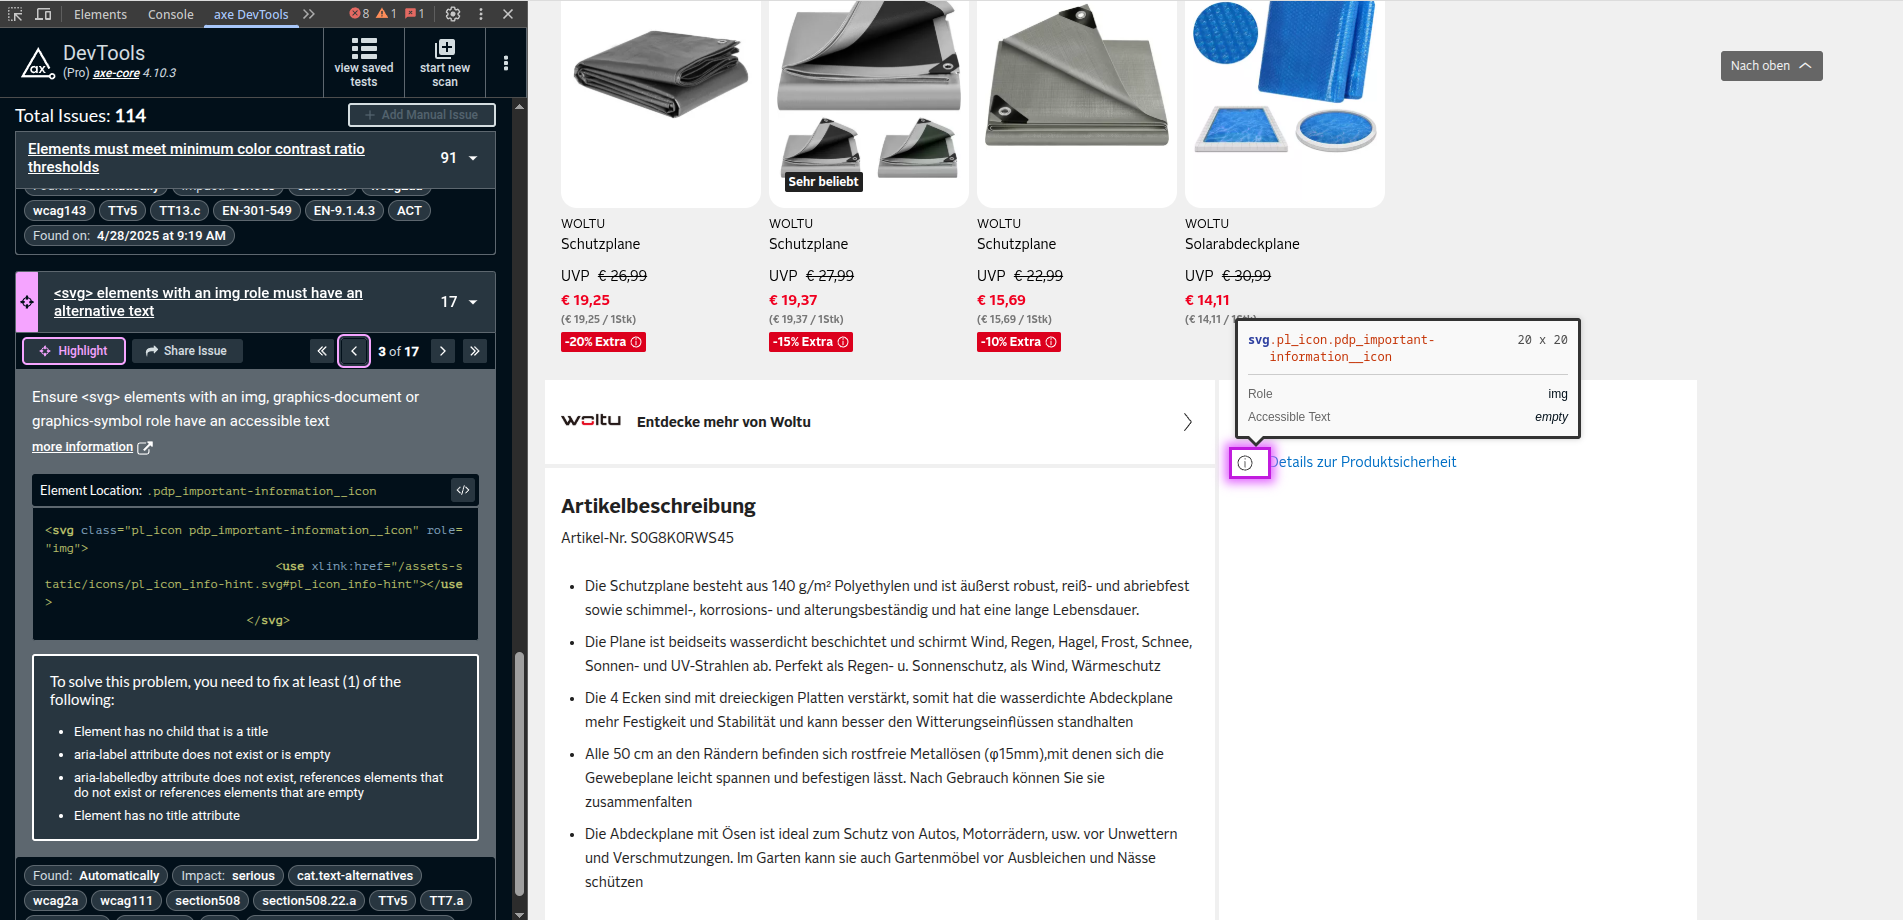
\includegraphics[width=\textwidth]{img/otto_svg-role-img-no-alt-text.png}
    \caption{Fehlender alternativer Text bei einem SVG mit der Rolle img}
\end{figure}

Das zweite Kriterium ist 1.4.3 "Mindestkontrast". Dabei handelt es sich um Kontrastprobleme zwischen Text und Hintergrund. Betroffen sind davon die Texte im Menü, einige Überschriften und Stichpunkte und Buttons auf der Startseite.
\begin{figure}[H]
    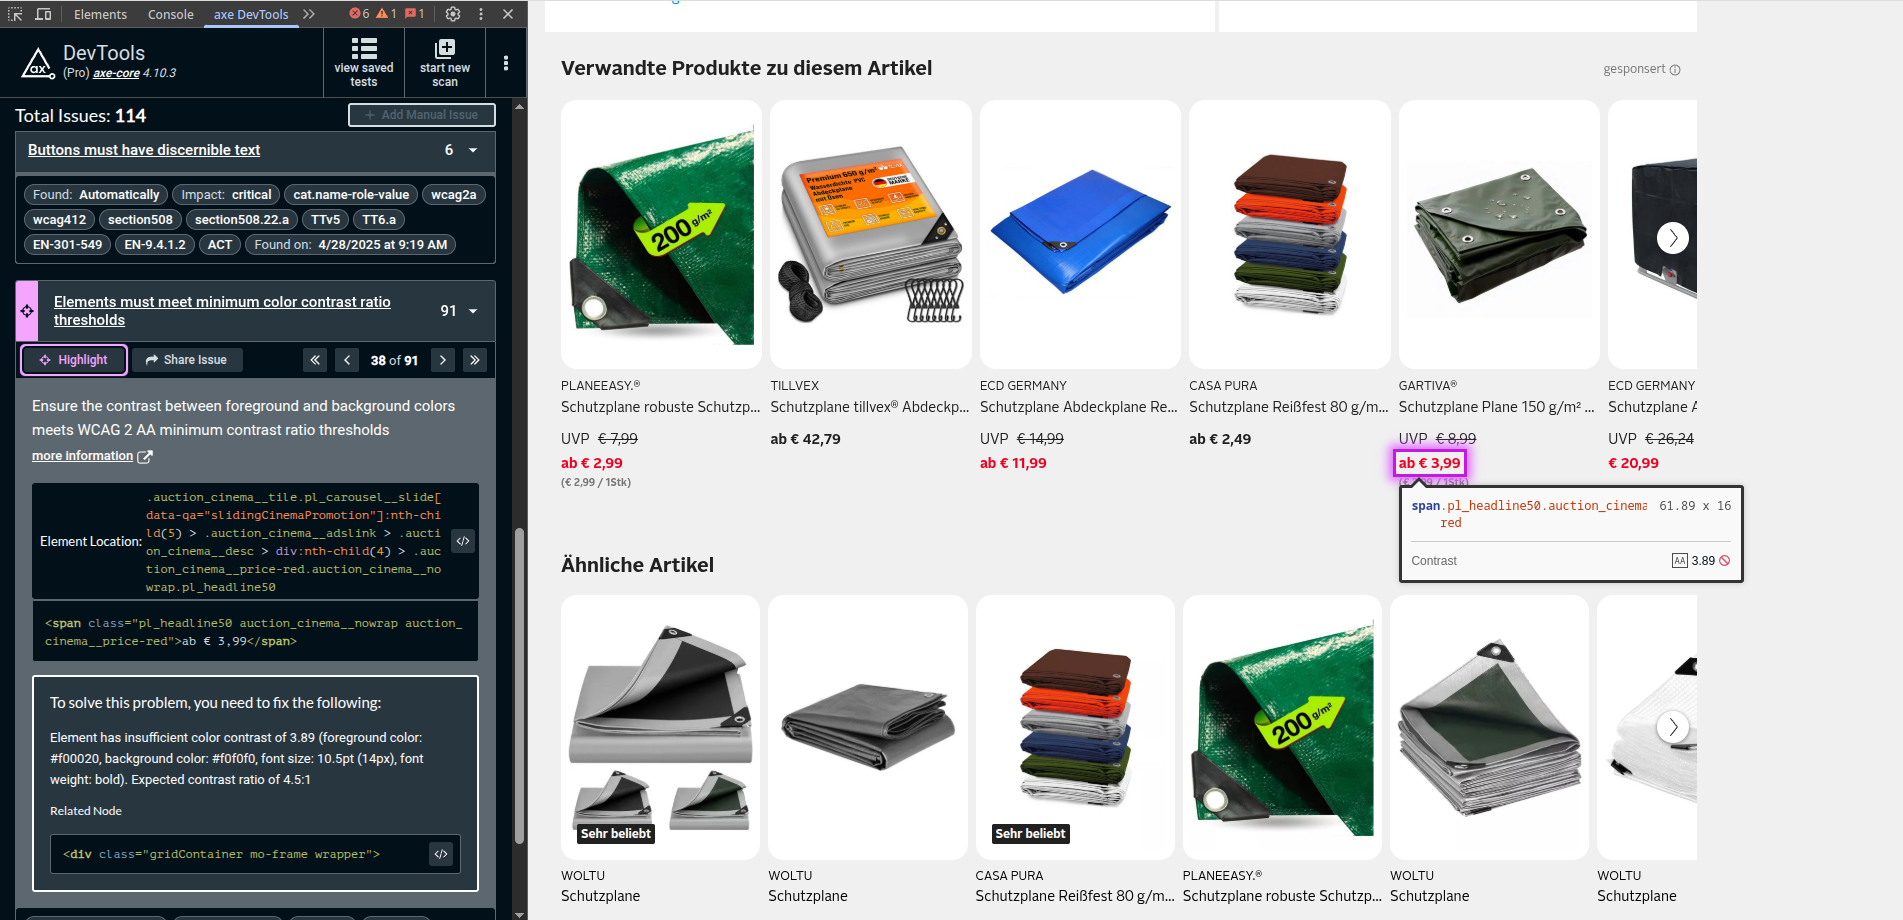
\includegraphics[width=\textwidth]{img/otto_failed-minimum-contrast.png}
    \caption{Kontrastprobleme auf der Startseite}
\end{figure}

Ein weiteres drittes Kriterium, welches häufig verletzt wurde, ist im Fokus sichtbar. Der Fokus wurde, wie bei den anderen Seiten auch, manuell getestet. Es ist schon beachtlich, wie oft der Fokus auf der Seite verschwindet und erst nach zwei bis drei Tabstops wieder auftaucht. Das ist ein Verstoß gegen Kriterium 2.4.7 "Fokus sichtbar".

Das letzte Kriterium ist 4.1.2 "Name, Rolle, Wert". Dabei handelt es sich um die korrekte Benennung der Elemente. Hier sind auch wieder die Buttons betroffen, die keinen zugänglichen Namen haben. Unter anderem betrifft es auch wieder einen Button, um den Slider weiter zu bewegen - wie bei Vodafone auch. 
\begin{figure}[H]
    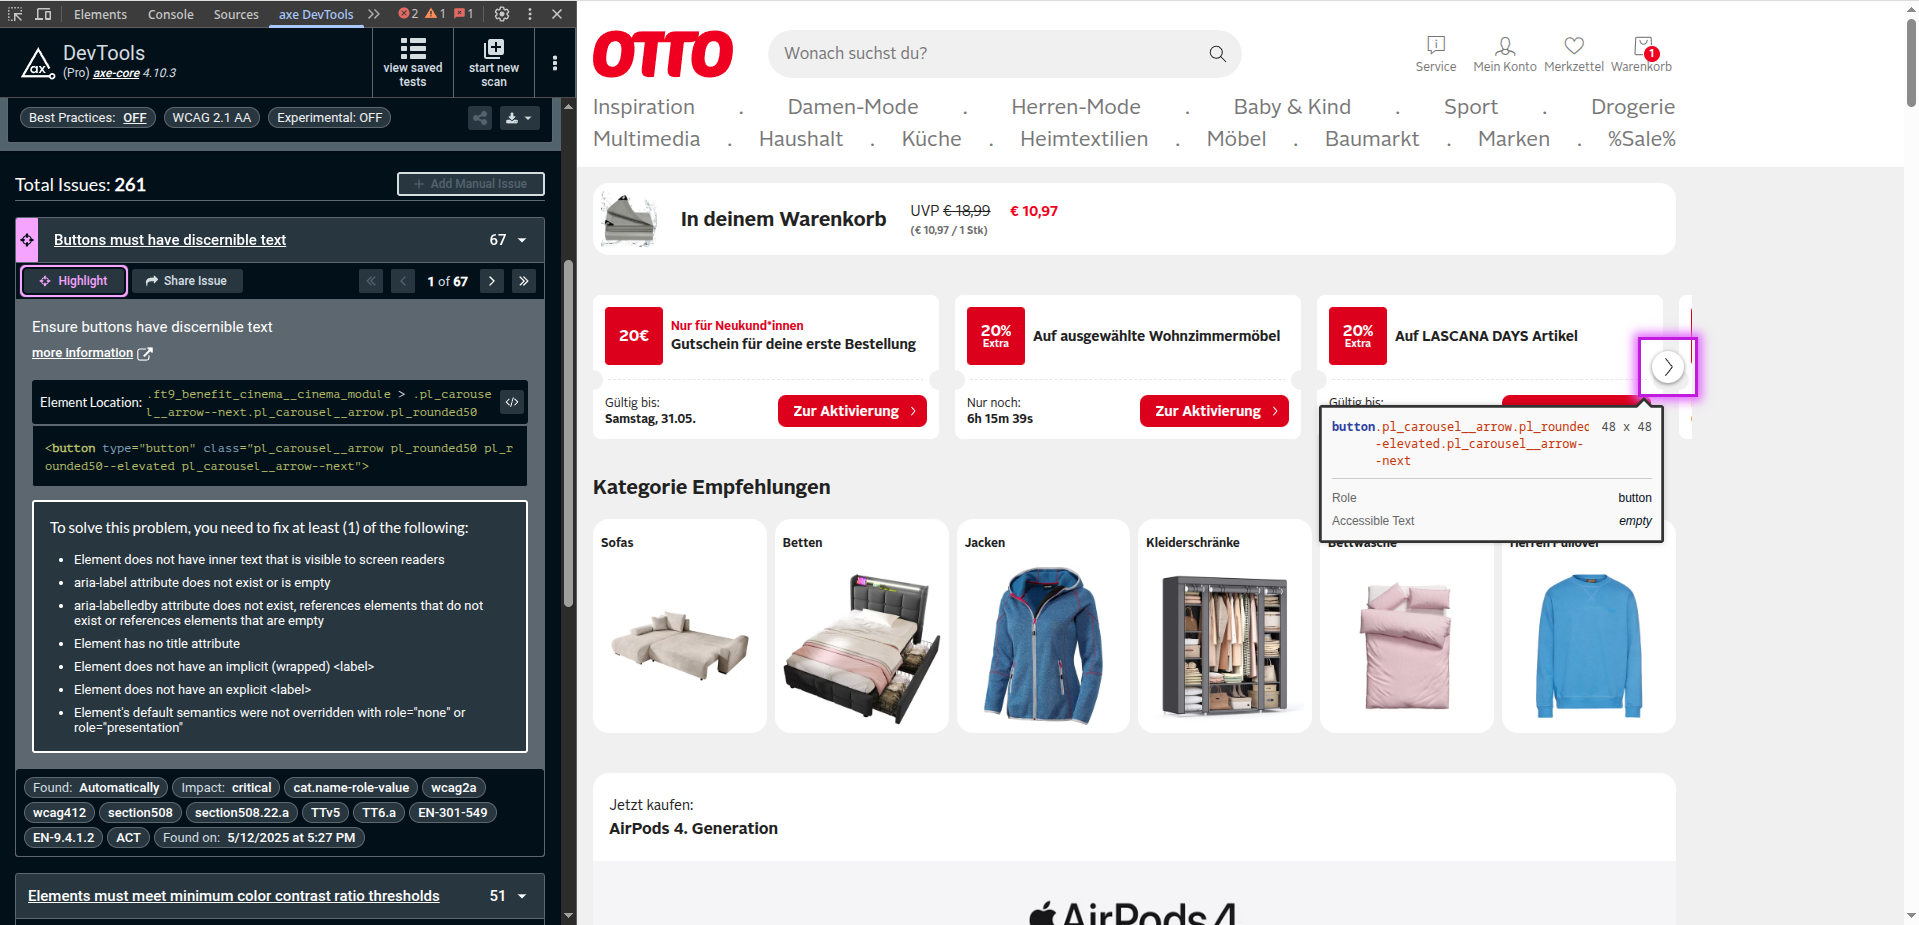
\includegraphics[width=\textwidth]{img/otto_button-slider-no-aria-label.png}
    \caption{Fehlendes Label bei einem Link}
\end{figure}

Die Fehler ziehen sich von der Startseite bis zu den Unterseiten, wie die Produktseiten. In der Gesamtbetrachtung (Abbildung 4.40) ist die Menge an Fehlern sehr gut zu erkennen.

\begin{figure}[H]
\begin{tikzpicture}
\begin{axis}[
    width=\textwidth,
    height=10cm,
    ybar,
    bar width=12pt,
    xlabel={WCAG-Kriterium},
    ylabel={Fehleranzahl},
    symbolic x coords={ 9.1.1.1, 9.1.3.1, 9.1.4.3, 9.2.4.1, 9.2.4.6, 9.2.4.7, 9.3.3.2, 9.4.1.2 },
    xtick=data,
    x tick label style={rotate=45, anchor=east},
    ymin=0,
    ymax=350,
    enlarge x limits=0.1,
    legend style={cells={anchor=west}, legend pos=north east},
    nodes near coords,
    nodes near coords style={font=\scriptsize},
]
\addplot table[x=WCAG-Kriterium,y=Fehleranzahl_axe,col sep=tab]{csv/output/wcag_analyse_Otto_xxxx.csv};
\addplot table[x=WCAG-Kriterium,y=Fehleranzahl_WAVE,col sep=tab]{csv/output/wcag_analyse_Otto_xxxx.csv};
\legend{axe,WAVE}
\end{axis}
\end{tikzpicture}
\caption{Auswertung Analyse Otto}
\end{figure}
